\documentclass[conference,onecolumn]{IEEEtran}
\usepackage[T1]{fontenc}
\usepackage{mathptmx}
\usepackage{amsmath,amssymb,graphicx,booktabs,array}
\usepackage{url}
\usepackage[hidelinks,hypertexnames=false]{hyperref}
\usepackage{placeins}
\usepackage{float}
\usepackage{capt-of}
\usepackage{multicol}
% Preserve IEEE conference column geometry while allowing inline wide bands.
\setlength{\columnsep}{0.25in}
\setlength{\multicolsep}{6pt}
\setlength{\intextsep}{7pt}
\raggedbottom
\newcommand{\startcolumns}{\begin{multicols}{2}\raggedcolumns}
\newcommand{\stopcolumns}{\end{multicols}}
\hypersetup{pdftitle={Semantic Analysis of Counterfactuals: Quality Under Transformations and Adaptive Benchmarking},pdfauthor={Milana Karimova, Sharaf Feyzullayev, Farah Feyzullayev, Jeyhuna Sevdiyeva, Nicat Aghayev}}
\newcommand{\artifactpath}[1]{\path{#1}}
\newcommand{\sacauthor}[2]{%
\begin{minipage}[t]{.31\textwidth}
\centering
\textbf{#1}\\[-.2ex]
{\footnotesize AI Academy,}\\[-.2ex]
{\footnotesize National Intelligence Center of Azerbaijan}\\[-.2ex]
{\scriptsize #2}
\end{minipage}}
% Course-report branding, not a claim of institutional endorsement.
\title{\makebox[\textwidth][c]{%
\makebox[.31\textwidth][c]{
\includegraphics[height=9mm,width=.29\textwidth,keepaspectratio]{figures/logos/AZCON_logo.png}}%
\makebox[.31\textwidth][c]{
\includegraphics[height=9mm,width=.29\textwidth,keepaspectratio]{figures/logos/naic_logo.png}}%
\makebox[.31\textwidth][c]{
\includegraphics[height=9mm,width=.29\textwidth,keepaspectratio]{figures/logos/academy_logo.png}}}\\[1.5mm]
\rule{.96\textwidth}{0.4pt}\\[3mm]
\makebox[\textwidth][c]{%
\begin{minipage}[c]{.10\textwidth}
\centering
\includegraphics[height=14mm,width=\linewidth,keepaspectratio]{figures/logos/sac_qutab_logo.png}
\end{minipage}\hspace{.01\textwidth}%
\begin{minipage}[c]{.87\textwidth}
\centering\LARGE Semantic Analysis of Counterfactuals:\\
Quality Under Transformations and Adaptive Benchmarking
\end{minipage}}}
% Team-supplied names/emails; affiliation confirmed by the user.
\author{%
\makebox[\textwidth][c]{%
\sacauthor{Milana Karimova}{milana.karimova25@aiacademy.edu.az}\hfill
\sacauthor{Sharaf Feyzullayev}{sheref.feyzullayev25@aiacademy.edu.az}\hfill
\sacauthor{Farah Feyzullayev}{fereh.feyzullayev25@aiacademy.edu.az}}\\[1.4ex]
\makebox[\textwidth][c]{%
\sacauthor{Jeyhuna Sevdiyeva}{ceyhune.sevdiyeva25@aiacademy.edu.az}\hspace{.045\textwidth}
\sacauthor{Nicat Aghayev}{nicat.agayev25@aiacademy.edu.az}}}
\begin{document}
\maketitle
\startcolumns
\begin{abstract}
\input{sections/00_abstract.tex}
\end{abstract}
\begin{IEEEkeywords}
Remote sensing, EuroSAT, transformation sensitivity, representation stability, failure detection, reproducibility.
\end{IEEEkeywords}
\input{sections/01_introduction.tex}
\input{sections/02_related_work.tex}
\input{sections/03_method.tex}
\section{Experimental Setup}\label{sec:setup}

\subsection{Dataset and four-way split}

The study uses EuroSAT RGB \cite{eurosat}: 27,000 labelled 64-by-64 patches covering ten land-use/land-cover classes. Table \ref{tab:split} reports the counts in the dataset manifest. Class stratification maintains class coverage across partitions, while content grouping keeps detected duplicates together. The split seed is 20260831. Exact and perceptual duplicates are grouped using \path{content-dhash-bktree-v1}, with a difference-hash Hamming threshold of four.

\begin{table}[H]
\centering
\caption{Four-way split by image and content group. Groups are defined by exact and near-duplicate content, without geographical separation.}\label{tab:split}
\begin{tabular}{lrr}
\toprule
Partition & Images & Groups \\
\midrule
Train & 16,200 & 15,246 \\
Validation & 4,050 & 4,050 \\
Calibration & 2,700 & 2,692 \\
Final Test & 4,050 & 4,050 \\
\bottomrule
\end{tabular}

\end{table}


Training contains 16,200 images; validation and final test each contain 4,050; calibration contains 2,700. Each partition has a defined role. Training updates model weights and supplies same-class amplitude-mixing donors. Validation selects checkpoints and fits the different-class-control ECDF. Calibration fits the failure detectors. Final test measures performance after those choices are fixed. Checkpoint selection and control normalization share one validation partition, while detector fitting and evaluation use separate data.

Final-test sources form 4,050 distinct content-based groups. Validation also has 4,050 groups; calibration has 2,692 and training has 15,246. Grouping prevents the defined exact and near-duplicate relationships from crossing partitions. It does not provide a country-, acquisition-, or region-held-out evaluation. Class counts range from 300 to 450 in final test; Appendix \ref{app:counts} gives the full allocation. Each final-test source supplies three families with four levels per family, including sham. The resulting 48,600 stored pairs per model/seed contain 36,450 non-sham pairs before the clean-correct filter.

\subsection{Models, pretraining, and optimization}

ResNet-50 and ViT-Small/16 are each trained with seeds 17, 29, and 43. Table \ref{tab:models} specifies the variants and representation layers. Both use supervised ImageNet-1k initialization, with the original classification head replaced for ten EuroSAT classes. The ViT checkpoint is the AugReg variant \cite{augreg,vitcard}; the ResNet checkpoint is the \path{tv_in1k} variant \cite{rescard}. Their pretraining recipes differ, so the model comparison includes both architecture and initialization effects.

\stopcolumns
\noindent
\begin{minipage}{\textwidth}
\centering
\captionof{table}{Model variants and training settings. Parameter counts include the ten-class head. Differences in pretraining and hardware limit attribution of performance gaps to architecture.}\label{tab:models}
\begin{tabular}{lll}\toprule
Field & ResNet-50 & ViT-Small/16 \\\midrule
timm variant & \texttt{resnet50.tv\_in1k} & \texttt{vit\_small\_patch16\_224.augreg\_in1k} \\
Trainable parameters & 23,528,522 & 21,669,514 \\
Representation & Pre-logit global average pool & Final normalized CLS token \\
Representation dimensions & 2,048 & 384 \\
Input / pretraining & $224\times224$ RGB / ImageNet-1k & $224\times224$ RGB / ImageNet-1k \\
Learning rate & $3\times10^{-4}$ & $5\times10^{-4}$ \\
Training device & H100 80GB & A100 MIG 3g.20gb \\
Training seeds & 17, 29, 43 & 17, 29, 43 \\\bottomrule
\end{tabular}
\end{minipage}
\par\startcolumns

All backbone parameters are fine-tuned. The common training recipe uses AdamW, weight decay 0.05, effective global batch size 64, a per-device batch of 32 and two gradient-accumulation steps on one device. Learning rates are \(3\times10^{-4}\) for ResNet-50 and \(5\times10^{-4}\) for ViT-Small/16. The schedule has two warm-up epochs followed by cosine decay toward 0.01 times the initial learning rate. Training is capped at 50 epochs. Checkpoint selection maximizes validation macro-F1 with minimum improvement 0.0001 and early-stopping patience ten epochs.

Training augmentation consists of deterministic horizontal and vertical flips, each with probability 0.5. There is no intervention-based augmentation, label smoothing, or frozen backbone in this executed recipe. Native tensors are resized and ImageNet-normalized as described in Section \ref{sec:method}. Mixed precision resolved to bfloat16. Deterministic configuration and recorded seeds improve repeatability, but do not imply bitwise equality across different devices and software versions.

The selected checkpoints occurred at one-based epochs 39, 48, and 42 for ResNet-50, and 38, 12, and 5 for ViT-Small/16. All six runs enter the comparison, preserving the observed variability of each training recipe. Final-test outcomes were not used to restart or tune the runs.

\subsection{Hardware and frozen evaluation}

ResNet training ran on an NVIDIA H100 80GB, whereas ViT training ran on an NVIDIA A100-SXM4-40GB MIG 3g.20gb instance. Their recorded training software also differs: PyTorch 2.13.0/CUDA 13.0 for ResNet and PyTorch 2.6.0+cu124 for ViT. Training wall times therefore cannot establish relative architectural efficiency. Final inference used the frozen A100 preflight configuration. The supporting audit retains the per-run metadata and checkpoint identifiers.

Before final-test evaluation, SHA-256 digests recorded the six checkpoints, run configurations, pair manifests, condition-selection policy, validation ECDFs, and calibration detectors. These identifiers allow later checks that the evaluated inputs match the frozen choices. All models and seeds use the same pair manifest. The active two-model campaign retains the base configuration identifier needed to trace the earlier ResNet runs.

Report generation required a vocabulary repair, and a later audit identified incorrect representation hashes in five historical report-index entries. The underlying six evaluation files were checked against their own indices and statistical sources before preparing the figures. Appendix \ref{app:provenance} records both incidents and the separate attention-visualization issue; original evaluations remain unchanged.

\subsection{Statistical estimands and uncertainty}

The primary within-model contrasts subtract mild from severe responses for label inconsistency, JS divergence, and normalized representation instability. Matching source images within each family measures the dose response on a fixed sample. Positive values mean greater instability at the severe setting. The three seed-level effects are summarized by their mean and sample standard deviation (SD, denominator \(n-1\)). SD describes variation across trained runs. The bootstrap confidence intervals (CIs) below quantify a different source of uncertainty: variation from resampling the evaluated source groups.

The primary statistics use 2,000 source-group bootstrap replicates and percentile 95\% CIs, with base seed 20260901 and deterministic offsets. All conditions from a sampled source group remain together because transformed versions of the same image are related observations. For RQ3, both detectors use the same resampled clean-correct groups, preserving the paired comparison. The intervals are conditional on the trained model and fitted detector. They exclude variation from detector refitting, a new calibration set, or a new geographical split.

The cross-model normalized-instability contrast is the ViT severe-minus-mild effect minus the ResNet effect, matched on source and training-seed identifier. A negative value indicates a smaller dose response for ViT on this normalized scale. The aggregate pairwise result averages over the three families and frozen seeds and uses a two-level bootstrap that resamples training seeds and source groups. Only three seeds provide evidence about training variability, limiting the interpretation of this interval beyond the observed runs.

The implementation applies Holm correction over configured model-pair contrasts within each seed/family, and separately over the aggregate model-pair summaries. Only one model pair is active, so each correction family contains one test. The procedure does not jointly correct across all families, seeds, or RQ3 intervals. A separate exploratory family contains 36 defined group-wise Wilcoxon tests across six runs, three families, and two metrics, with Benjamini--Hochberg false-discovery-rate level 0.05. Class-wise summaries are descriptive and are outside both test families.

Some stored Wilcoxon p-values are numerically zero and are reported as \(p<0.001\), alongside effect sizes and uncertainty intervals. The supplementary within-run JS--ECDF correlations are post-hoc descriptive summaries of saved outputs and are separate from the primary tests. These summaries can be reproduced from the saved outputs without new training or final-test inference.

\section{Results}\label{sec:results}

\subsection{Clean performance and seed variability}

ResNet-50 achieves higher clean accuracy with less variation across seeds under the executed recipes. Mean final-test accuracy is 98.63\% for ResNet-50 and 96.77\% for ViT-Small/16, with sample SDs of 0.04 and 1.21 percentage points, respectively. Macro-F1 follows the same ordering (Table \ref{tab:clean}). These clean scores provide the reference for measuring transformation effects.

\stopcolumns
\noindent\begin{minipage}[t]{\dimexpr(\textwidth-\columnsep)/2\relax}
\begin{table}[H]
\centering
\caption{Clean final-test performance, mean $\pm$ sample SD across three seeds. Accuracy and macro-F1 are percentages; ECE, Brier and NLL use their native scales. Each run evaluates 4,050 sources. Bold marks the better model for each metric; higher is better for accuracy and macro-F1, while lower is better for ECE, Brier and NLL.}\label{tab:clean}
\begin{tabular}{lrr}
\toprule
Metric & ResNet-50 & ViT-Small/16 \\
\midrule
Acc. (\%) & \textbf{98.63 $\pm$ 0.04} & 96.77 $\pm$ 1.21 \\
Macro-F1 (\%) & \textbf{98.58 $\pm$ 0.03} & 96.66 $\pm$ 1.24 \\
ECE & \textbf{0.0080 $\pm$ 0.0005} & 0.0116 $\pm$ 0.0042 \\
Brier & \textbf{0.0218 $\pm$ 0.0009} & 0.0502 $\pm$ 0.0165 \\
NLL & \textbf{0.0577 $\pm$ 0.0038} & 0.1064 $\pm$ 0.0220 \\
\bottomrule
\end{tabular}

\end{table}

\end{minipage}\hfill\begin{minipage}[t]{\dimexpr(\textwidth-\columnsep)/2\relax}
ResNet's mean expected calibration error (ECE) is 0.0080, versus 0.0116 for ViT, using 15 equal-width confidence bins. Brier score and negative log-likelihood also favor ResNet. Calibration and accuracy nevertheless measure different properties: the lowest-accuracy ViT seed has ECE 0.0067, lower than that of the highest-accuracy ViT seed. A small aggregate calibration gap can coexist with lower accuracy. ECE also depends on binning and the evaluated population \cite{calibration}.

ViT seed 17 attains 98.15\% clean accuracy, while seeds 29 and 43 attain 96.25\% and 95.90\%. All three contribute to the mean. The selected validation epochs and learning curves document this variation across runs, although they do not identify its cause.
\end{minipage}\par\startcolumns

\subsection{RQ1: sensitivity depends strongly on the transformation family}

Resolution reduction produces the largest deterioration on the tested dose grid. ResNet accuracy falls from 87.89\% at mild reduction to 49.47\% at moderate and 12.94\% at severe reduction. ViT falls from 92.89\% to 77.17\% and 43.00\%, respectively. ViT therefore retains higher accuracy at all three tested resolution levels despite its lower clean accuracy. Figure \ref{fig:prediction} shows accuracy alongside JS divergence, separating label correctness from changes in the probability distribution.

\stopcolumns
\noindent\begin{minipage}{\textwidth}
\centering
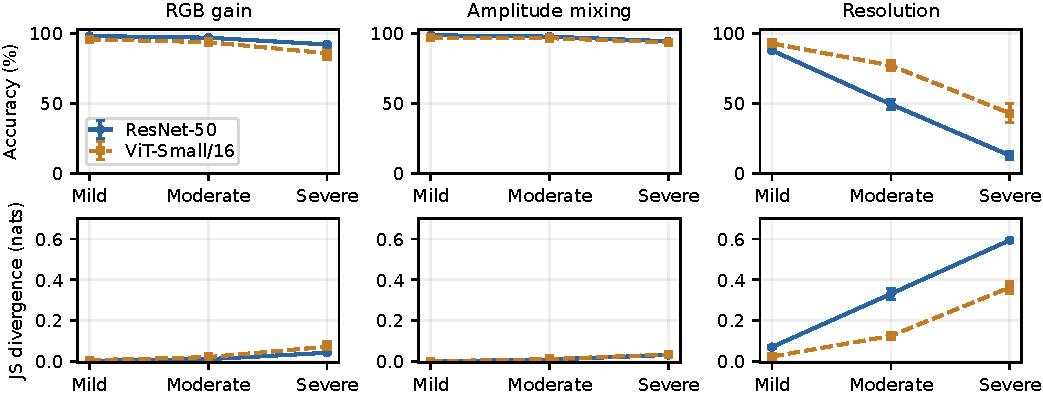
\includegraphics[width=\textwidth]{figures/prediction_response_compact.pdf}
\captionof{figure}{Prediction response across the three frozen doses of each family. Points show means across three seeds, and error bars show sample SD. Each condition uses 4,050 sources per run. Lines connect the evaluated doses; intermediate severities were not measured.}\label{fig:prediction}
\end{minipage}
\par\startcolumns


ResNet retains the advantage under the other two families. Under severe RGB gains, accuracy is 92.14\% for ResNet and 85.85\% for ViT; under severe amplitude mixing, the means are 94.41\% and 93.59\%. Model performance must therefore be described by transformation family. The intervention scales are not perceptually matched, and severe resolution reduction may remove information needed to identify the original class.

Table \ref{tab:contrasts} reports severe-minus-mild effects for matched source images. ResNet's mean resolution JS increase is 0.5219 nats, a large change within the possible JS range of 0 to \(\log 2\). Its RGB-gain and amplitude-mixing increases are much smaller. Label inconsistency, distributional change, and normalized feature change have different units, so their numerical magnitudes should be interpreted within each metric.

\stopcolumns
\noindent\begin{minipage}{\textwidth}
\centering
\captionof{table}{Primary paired severe-minus-mild effects, mean $\pm$ sample SD across seeds. Positive values indicate increasing instability. JS uses natural logarithms; ECDF is on a 0--1 percentile scale. Each per-seed contrast uses the same 4,050 sources. Within each family, bold marks the lower sensitivity value; displayed ties are bold for both models.}\label{tab:contrasts}
\begin{tabular}{llrrr}
\toprule
Model & Family & $\Delta$ inconsistency (pp) & $\Delta$ JS (nats) & $\Delta$ ECDF \\
\midrule
ResNet-50 & RGB gain & \textbf{6.4527 $\pm$ 0.9056} & \textbf{0.0397 $\pm$ 0.0050} & \textbf{0.0028 $\pm$ 0.0008} \\
ResNet-50 & Amplitude mixing & \textbf{5.1276 $\pm$ 0.1918} & \textbf{0.0320 $\pm$ 0.0015} & \textbf{0.0015 $\pm$ 0.0003} \\
ResNet-50 & Resolution & 75.3086 $\pm$ 3.9397 & 0.5219 $\pm$ 0.0146 & 0.6131 $\pm$ 0.0361 \\
ViT-Small/16 & RGB gain & 11.1440 $\pm$ 3.3825 & 0.0660 $\pm$ 0.0220 & 0.0054 $\pm$ 0.0043 \\
ViT-Small/16 & Amplitude mixing & 5.8272 $\pm$ 0.2848 & 0.0335 $\pm$ 0.0008 & \textbf{0.0015 $\pm$ 0.0002} \\
ViT-Small/16 & Resolution & \textbf{51.3498 $\pm$ 6.6212} & \textbf{0.3376 $\pm$ 0.0354} & \textbf{0.0874 $\pm$ 0.0069} \\
\bottomrule
\end{tabular}

\end{minipage}
\par\startcolumns


The lowest dose can also produce a small accuracy increase. Mean mild amplitude-mixing accuracy is 98.73\% for ResNet and 97.13\% for ViT, slightly above their respective clean means. Accuracy can rise when corrections of initially wrong predictions outnumber correct-to-incorrect transitions. Label consistency records both kinds of changes. The observed increases are descriptive outcomes on this held-out partition; they do not establish that amplitude mixing would improve generalization if used during training.

\subsection{RQ2: normalized feature stability and prediction stability are not interchangeable}

Resolution reduction also produces the largest representation changes within each model (Figure \ref{fig:representation}). At severe reduction, ResNet's mean raw cosine similarity is 0.3929 and its ECDF instability is 0.6202; ViT's corresponding values are 0.5550 and 0.0876. The lower ViT ECDF value places its displacement at a lower percentile of its own different-class control distribution. Because the reference distributions are model-specific, the percentiles do not equate absolute distances in the 384- and 2,048-dimensional spaces.

\stopcolumns
\noindent\begin{minipage}{\textwidth}
\centering
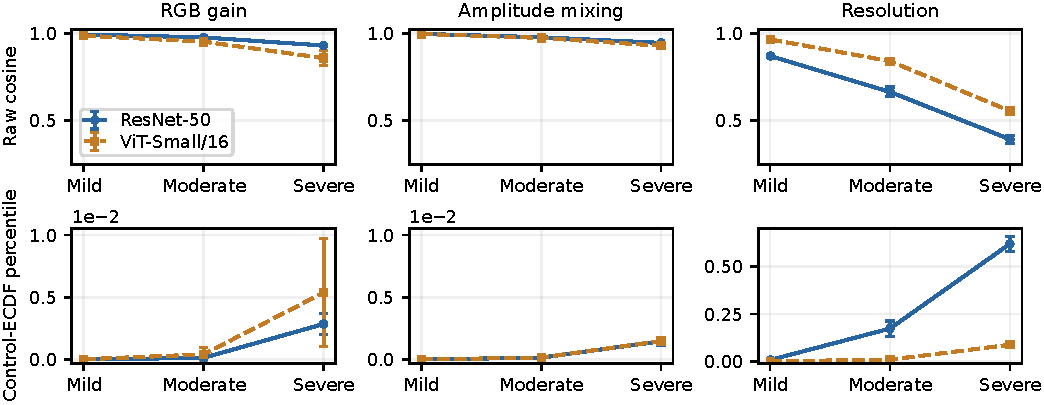
\includegraphics[width=\textwidth]{figures/representation_response_compact.pdf}
\captionof{figure}{Raw within-model cosine (top) and validation-control ECDF instability (bottom), shown as mean and sample SD across seeds. The bottom panels use different scales because RGB gain and amplitude mixing occupy the ECDF lower tail. Near-zero percentiles can coexist with changed predictions. Larger ECDF values indicate greater displacement relative to the run's controls.}\label{fig:representation}
\end{minipage}
\par\startcolumns


Under resolution reduction, the paired increase in normalized instability is 0.6131 $\pm$ 0.0361 for ResNet and 0.0874 $\pm$ 0.0069 for ViT (mean $\pm$ sample SD). Averaging the ViT-minus-ResNet difference-in-differences over all three families gives -0.1744, with a stored two-level bootstrap 95\% CI of [-0.1851, -0.1633]. The group-wise aggregate Wilcoxon result is reported as \(p<0.001\); its Holm family contains only the single active model pair. Resolution dominates this aggregate, so the average does not describe an equal effect across RGB gain, amplitude mixing, and resolution reduction.

Severe RGB gains illustrate why normalized feature stability and prediction stability can diverge. Mean ECDF instability is only 0.00285 for ResNet and 0.00537 for ViT, yet label consistency falls to 92.61\% and 86.77\%. Features can remain close relative to different-class controls while crossing a decision boundary. The raw-cosine panels in Figure \ref{fig:representation} retain within-model changes that are compressed near the ECDF floor.

Figure \ref{fig:scatter} relates confidence drop to normalized representation instability for individual pairs. Each panel contains 109,350 non-sham observations, pooling three seeds and nine conditions for 4,050 sources. In both models, a dense band near the ECDF floor spans a range of confidence changes. A low control percentile therefore does not determine the size of the confidence change. Sources appear repeatedly across seeds and conditions, so the points are dependent observations; the display does not support a causal interpretation.

\stopcolumns
\noindent\begin{minipage}{\textwidth}
\centering
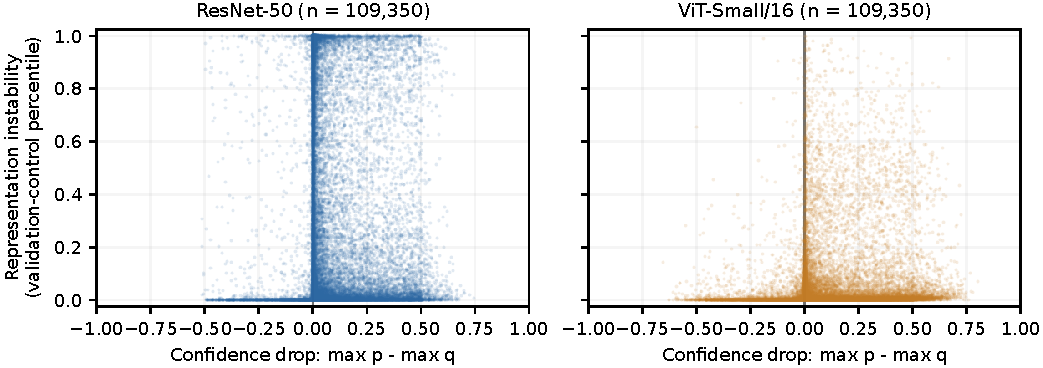
\includegraphics[width=\textwidth]{figures/confidence_representation_scatter_compact.pdf}
\captionof{figure}{Confidence drop and representation instability for all non-sham pairs: 109,350 observations per model (4,050 sources, nine conditions, three seeds). Positive horizontal values indicate a confidence decrease; negative values indicate an increase. The vertical coordinate is a validation-control percentile, not a failure probability. Both panels share scales and include clean errors. Sources recur across seeds and conditions, so observations are dependent. No correlation test is attached to this display.}\label{fig:scatter}
\end{minipage}
\par\startcolumns


The scatter includes initially incorrect predictions. RQ3 restricts evaluation to initially correct sources and tests whether the representation feature improves detection of their subsequent failures.

\subsection{RQ3: representation adds discrimination beyond the specified output baseline}

Adding normalized representation instability improves both AP and AUROC in every model/seed comparison. Mean paired AP gains are 0.432 $\pm$ 0.113 for ResNet and 0.402 $\pm$ 0.032 for ViT. Mean paired AUROC gains are 0.166 $\pm$ 0.087 and 0.114 $\pm$ 0.023. The $\pm$ values are sample SDs across three seeds. Table \ref{tab:detectors} gives all five score variants and the paired gains.

\stopcolumns
\noindent\begin{minipage}{\textwidth}
\centering
\captionof{table}{Failure-discrimination scores and paired gains, mean $\pm$ sample SD across three seeds. AP denotes average precision. Populations and prevalence differ by model/seed (Appendix~\ref{app:detector}); paired gains compare detectors on the same rows within each run. Within each model, bold marks the highest AP or AUROC among the five absolute score variants.}\label{tab:detectors}
\begin{tabular}{lrrrr}
\toprule
& \multicolumn{2}{c}{ResNet-50} & \multicolumn{2}{c}{ViT-Small/16} \\
Score / paired gain & AP & AUROC & AP & AUROC \\
\midrule
Confidence & 0.513 $\pm$ 0.102 & 0.819 $\pm$ 0.084 & 0.489 $\pm$ 0.028 & 0.867 $\pm$ 0.027 \\
Entropy & 0.513 $\pm$ 0.105 & 0.818 $\pm$ 0.085 & 0.498 $\pm$ 0.029 & 0.869 $\pm$ 0.026 \\
Output only & 0.507 $\pm$ 0.107 & 0.818 $\pm$ 0.085 & 0.496 $\pm$ 0.028 & 0.869 $\pm$ 0.026 \\
Output + representation & \textbf{0.939 $\pm$ 0.006} & \textbf{0.983 $\pm$ 0.001} & \textbf{0.898 $\pm$ 0.020} & \textbf{0.983 $\pm$ 0.007} \\
Representation only & 0.918 $\pm$ 0.008 & 0.966 $\pm$ 0.005 & 0.878 $\pm$ 0.032 & 0.955 $\pm$ 0.017 \\
$\Delta$ AP & 0.432 $\pm$ 0.113 & -- & 0.402 $\pm$ 0.032 & -- \\
$\Delta$ AUROC & -- & 0.166 $\pm$ 0.087 & -- & 0.114 $\pm$ 0.023 \\
\bottomrule
\end{tabular}

\end{minipage}
\par\startcolumns


Figure \ref{fig:detectors} shows the within-seed source-group bootstrap intervals for the paired gains. Every displayed interval lies above zero, although the twelve intervals do not provide simultaneous coverage.

\stopcolumns
\noindent\begin{minipage}{\textwidth}
\centering
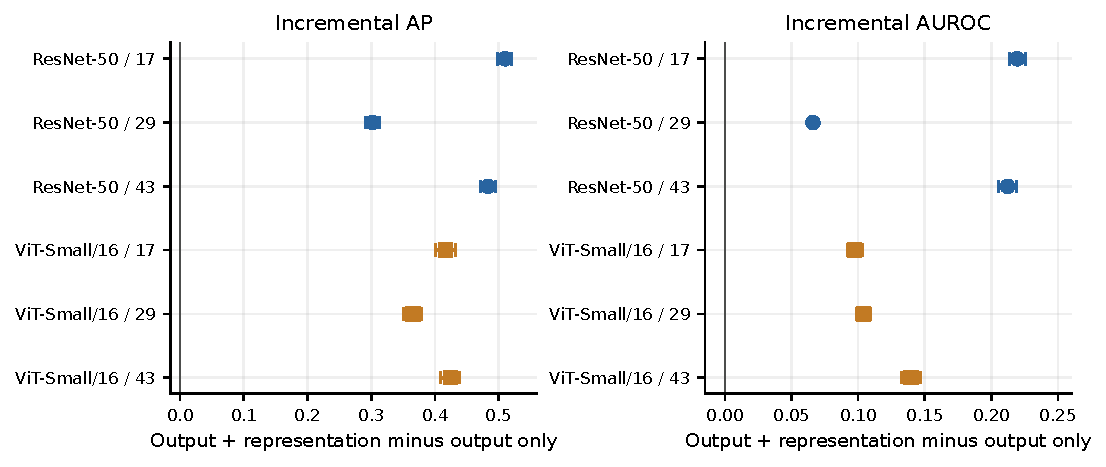
\includegraphics[width=\textwidth]{figures/detector_deltas.pdf}
\captionof{figure}{Incremental detector performance by training seed. Points show paired gains from adding representation to the two output features. Bars are stored 95\% source-group bootstrap CIs from 2,000 replicates, conditional on each trained model and fitted detector. Every interval excludes zero; coverage is individual rather than simultaneous.}\label{fig:detectors}
\end{minipage}
\par\startcolumns


The eligible population comprises 35,937--35,964 pairs per ResNet seed and 34,956--35,775 per ViT seed. Positive prevalence is 18.05--18.55\% for ResNet and 10.30--13.12\% for ViT. Both population size and prevalence depend on which sources each run classifies correctly before transformation and which then fail. Since AP depends on prevalence, the absolute scores do not provide a population-matched ranking of the models. Comparing the two detectors within each run holds the population fixed. Appendix \ref{app:detector} reports the exact counts and prevalence.

The representation-only score achieves mean AP of approximately 0.918 for ResNet and 0.878 for ViT. Adding the two output features raises the respective means to approximately 0.939 and 0.898. Much of the gain over the output-only baseline is therefore present in the representation score alone. The evidence supports this feature's value within the tested logistic model, without establishing a need for a more complex fusion architecture. Richer output-only baselines remain an open comparison.

The ResNet output baseline varies substantially across seeds: its AUROC is 0.765, 0.916, and 0.772 for seeds 17, 29, and 43. The augmented detector remains at approximately 0.982--0.985 across the same runs. The resulting gain is consequently smaller for seed 29, as reflected in the per-seed intervals and the SD of the paired gains.

The pooled detector task gives each source one pair in each of the nine conditions. Differences in condition difficulty, especially the high failure rate under resolution reduction, can contribute to pooled discrimination. Equal performance within every family, class, or severity cannot be inferred from that score. The saved condition-prevalence tables document the mixture, but the pooled summary does not supply condition-specific AUROC estimates. Detector calibration, operating thresholds, and performance under deployment shifts were also not established by this evaluation.

\subsection{Controls and class-wise behavior}

Sham conditions retain label consistency of one across all six runs, confirming that the identity processing paths preserve predicted labels. The check does not extend to semantic preservation under nonzero perturbations. Different-class controls supply the ECDF reference scale using known labels and content exclusions; their purpose is normalization rather than an independent adversarial stress test.

Figure \ref{fig:classes} breaks down severe-condition label consistency by the ten original classes. Each cell averages the same three seeds and includes all final-test sources in the class, including clean errors. The denominator therefore differs from RQ3. The resolution columns show substantial variation across classes that is concealed by a single model mean. All classes are shown, and the cell differences are descriptive; no class-wise significance tests were performed.

\stopcolumns
\noindent\begin{minipage}{\textwidth}
\centering
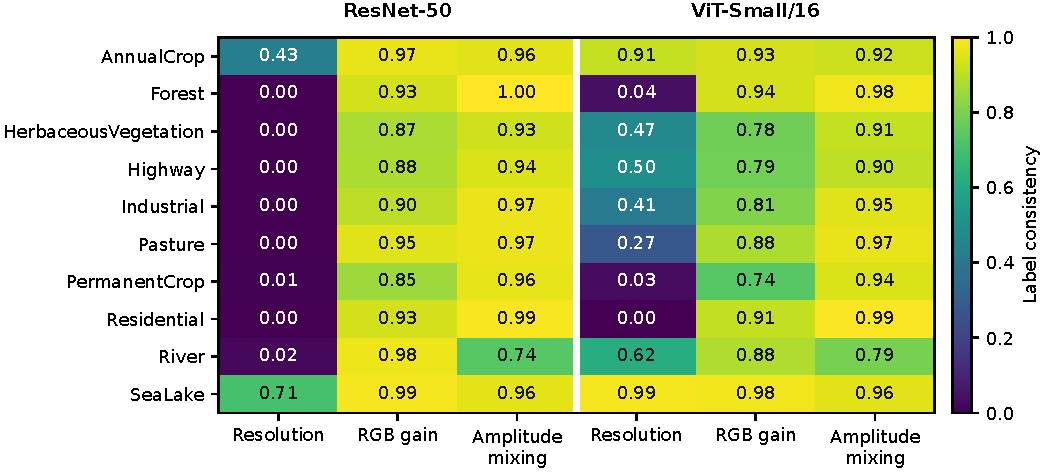
\includegraphics[width=\textwidth]{figures/class_heatmap_compact.pdf}
\captionof{figure}{Severe-condition label consistency by class, averaged across three seeds. Each cell includes all class sources, including clean errors. Consistency measures agreement with the clean prediction; accuracy would compare with the dataset label. The shared scale runs from zero (purple) to one (yellow), with rounded values printed in each cell. Class sample counts appear in Appendix~\ref{app:counts}. Cell differences are descriptive and have no class-wise significance tests.}\label{fig:classes}
\end{minipage}
\par\startcolumns


Appendix \ref{app:qualitative} illustrates four failures selected for high clean confidence and mild transformation severity. All four involve RGB gains and prediction switches between PermanentCrop and HerbaceousVegetation. Clean confidence exceeds 0.99 in each case, yet the transformed prediction is incorrect relative to the dataset label. The selection illustrates the failure definition without estimating its frequency. Appendix \ref{app:attention} presents the related attention rollout and documents its rendering repair.

\section{Discussion and Limitations}\label{sec:discussion}

\subsection{Model rankings depend on the tested change}

The model ranking depends on the change applied to the image. ResNet's clean-accuracy advantage coexists with a larger loss under resolution reduction, while ViT's resolution advantage does not extend to RGB gains. Averaging across families obscures these differences because resolution dominates the aggregate contrast in normalized instability. When the expected image changes are known, the family-specific responses provide the more relevant comparison.

Several factors could contribute to the observed ordering. The models differ in pretraining recipe, representation dimensionality, fine-tuning learning rate, software, and training hardware. Early stopping also selects widely separated ViT epochs. These factors were not varied independently, so the resolution result cannot be attributed solely to global attention. Isolating an architectural explanation would require controlling the training recipe and environment.

\subsection{Designed transformations and scene meaning}

The absence of human review limits the interpretation of prediction changes. Full-spectrum amplitude mixing can alter spatial structure as well as appearance, RGB clipping can change local cues, and downsampling can erase small objects or boundaries. Same-class donors and retained source phase constrain the operation, but a reviewer might still assign a different label afterward. Reported failures are measured relative to the source dataset labels.

Information loss is an alternative explanation to shortcut reliance, especially under severe resolution reduction. The mild RGB-gain examples in Appendix \ref{app:qualitative} show that even high clean confidence can precede a changed, incorrect prediction. Their deliberate selection leaves both frequency and causal explanation unresolved. Attention rollout describes the model's attention pattern but cannot determine whether the original label remains appropriate.

\subsection{What the detector gains establish}

The positive within-run gains support adding normalized feature displacement to transformed uncertainty and entropy for the specified task. Richer output features, including clean/transformed JS and probability-vector differences, remain untested and might recover some of the same information. Their evaluation would need to be identified as a separate analysis, with the original frozen baseline retained as the reference.

The need for a clean reference image restricts the evaluated detector to paired benchmark diagnosis. Monitoring incoming satellite images would require a different evaluation design. The present task also excludes existing clean errors and pools conditions with different failure rates. AP and AUROC assess ranking within that population; they do not supply a deployment false-alarm rate, calibrated failure probability, or operating threshold.

\subsection{Sampling and uncertainty}

Content-based grouping addresses the exact and near-duplicate relationships defined by the implementation but does not enforce geographical separation. The study uses one RGB benchmark without an independent domain, season, or multispectral evaluation. Three training seeds provide a limited sample of optimization variability. Additional bootstrap resamples cannot supply evidence from more training runs or test domains.

Seed SD describes dispersion across trained runs, while per-seed source-group bootstrap CIs describe finite-source variation conditional on a checkpoint and fitted detector. The aggregate two-level interval also resamples the three available seeds, providing limited evidence about less common training outcomes. Multiple-testing corrections apply only to the families defined in the setup. Class heatmaps and post-hoc correlations consequently retain a descriptive interpretation.

\subsection{Planned versus executed study}

Table \ref{tab:deviations} records the main changes from the proposal and older template. Model variants, split roles, transformation definitions, and results follow the executed study. Optional spatial, masked-autoencoder, multispectral, and gamma extensions were not evaluated. The reporting repairs and visualization issue are documented separately in Appendix \ref{app:provenance}.

\stopcolumns
\noindent
\begin{minipage}{\textwidth}
\centering
\captionof{table}{Differences between the proposal or earlier template and the executed study.}\label{tab:deviations}
\begin{tabular}{p{.19\textwidth}p{.31\textwidth}p{.41\textwidth}}\toprule
Decision & Earlier plan/template & Executed study reported here \\\midrule
Models & ResNet-18 and compact DeiT/ViT variants; broader operational model matrix & ResNet-50 and ViT-Small/16; seeds 17, 29, 43 \\
Partition roles & Earlier split descriptions & Four fixed partitions, with separate detector calibration and final test \\
Semantic review & Planned human acceptance/adjudication & No human semantic review; all predeclared conditions retained by design \\
Fourier operator & Earlier masked-amplitude descriptions & Full-spectrum convex amplitude mixing, same-class training donor \\
Optional extensions & Spatial, MAE, multispectral and gamma directions & Not executed; no corresponding empirical claims \\
Report generation & Automated final artifact generation & Vocabulary repair; later report-index provenance defect independently audited \\\bottomrule
\end{tabular}
\end{minipage}
\par\startcolumns

Human review of label preservation on a prespecified sample would clarify the meaning of the observed failures. Additional seeds and externally held-out domains would address training and sampling uncertainty. Richer output baselines would test how much of the paired signal can be recovered without representation access. Each follow-up requires a new evaluation design that preserves the current final test as a completed experiment.

\section{Reproducibility}\label{sec:repro}

The report package contains editable English sections, LaTeX tables, figures, generation scripts, and a ledger linking claims to evidence. Quantitative figures are rebuilt from saved evaluations and statistics. Gallery inputs were recovered from the backup and checked against recorded hashes. The audit links each of the six checkpoints to its evaluation inputs, representation rows, and detector scores. Original evidence, including the historical report index, is preserved.

Reproduction requires different resources at each level. Rebuilding the document uses the supplied LaTeX sources and figure assets. Recomputing the analysis uses the frozen outputs. Repeating the experiment additionally requires raw EuroSAT images, matching pretrained weights, resolved configuration, software environment, training code, and appropriate hardware. The report audit does not certify that every external dependency is present in the project directory. Authenticated manifests and verified retrieval instructions are needed for large binary resources, with licensing and access checked before publication. The report README describes the available inputs and the scope of each script.

The project repository cited in the abstract provides the public reproducibility entry point. The publication release is identified by \path{v1.0-final}; the historical research baseline remains identified by \path{sac-campaign-v1-final}. Appendix \ref{app:provenance} provides protocol and configuration identifiers.

\section{Conclusion}

On the tested EuroSAT RGB transformations, neither model has the highest accuracy in every condition. ResNet-50 has higher mean clean accuracy (98.63\% versus 96.77\%), while ViT-Small/16 retains more accuracy under severe resolution reduction (43.00\% versus 12.94\%). Prediction and representation stability also describe different responses: a transformed representation can remain close relative to different-class controls while the predicted label changes. Raw cosine and the ECDF percentile make these scales of feature change explicit.

For clean-correct, non-sham pairs, adding normalized representation instability to transformed uncertainty and entropy improves AP and AUROC in all six runs. Mean AP gains are 0.432 for ResNet and 0.402 for ViT. The paired representation feature therefore improves failure ranking beyond the specified output baseline on this benchmark. Extending the conclusion requires evidence about semantic preservation and performance on independent domains.

\section{Tools and Acknowledgements}

The experiment artifacts record use of PyTorch, torchvision, timm, NumPy, SciPy, scikit-learn, Pillow, Matplotlib, and Weights \& Biases. OpenAI Codex assisted with source inspection, audit and figure scripts, drafting, language revision, reference checking, and LaTeX preparation. The team supplied author details and affiliation. The authors remain responsible for checking the claims and approving submission. Report preparation involved no human semantic annotation, new training, detector fitting, or full final-test inference. A post-hoc forward pass on the two recorded inputs generated the corrected attention figure described in Appendix \ref{app:attention}.

\FloatBarrier
\begin{thebibliography}{16}
\bibitem{eurosat} P. Helber, B. Bischke, A. Dengel, and D. Borth, ``EuroSAT: A novel dataset and deep learning benchmark for land use and land cover classification,'' \emph{IEEE J. Sel. Topics Appl. Earth Observ. Remote Sens.}, vol. 12, no. 7, pp. 2217--2226, 2019.
\bibitem{resnet} K. He, X. Zhang, S. Ren, and J. Sun, ``Deep residual learning for image recognition,'' in \emph{Proc. CVPR}, 2016, pp. 770--778.
\bibitem{vit} A. Dosovitskiy \emph{et al.}, ``An image is worth 16x16 words: Transformers for image recognition at scale,'' in \emph{Proc. ICLR}, 2021.
\bibitem{augreg} A. Steiner, A. Kolesnikov, X. Zhai, R. Wightman, J. Uszkoreit, and L. Beyer, ``How to train your ViT? Data, augmentation, and regularization in vision transformers,'' \emph{Trans. Mach. Learn. Res.}, 2022.
\bibitem{corruptions} D. Hendrycks and T. Dietterich, ``Benchmarking neural network robustness to common corruptions and perturbations,'' in \emph{Proc. ICLR}, 2019.
\bibitem{shortcut} R. Geirhos \emph{et al.}, ``Shortcut learning in deep neural networks,'' \emph{Nature Machine Intelligence}, vol. 2, pp. 665--673, 2020, doi: 10.1038/s42256-020-00257-z.
\bibitem{texture} R. Geirhos, P. Rubisch, C. Michaelis, M. Bethge, F. A. Wichmann, and W. Brendel, ``ImageNet-trained CNNs are biased towards texture; increasing shape bias improves accuracy and robustness,'' in \emph{Proc. ICLR}, 2019.
\bibitem{fda} Y. Yang and S. Soatto, ``FDA: Fourier domain adaptation for semantic segmentation,'' in \emph{Proc. CVPR}, 2020, pp. 4085--4095.
\bibitem{baseline} D. Hendrycks and K. Gimpel, ``A baseline for detecting misclassified and out-of-distribution examples in neural networks,'' in \emph{Proc. ICLR}, 2017.
\bibitem{calibration} C. Guo, G. Pleiss, Y. Sun, and K. Q. Weinberger, ``On calibration of modern neural networks,'' in \emph{Proc. ICML}, PMLR vol. 70, 2017, pp. 1321--1330.
\bibitem{cka} S. Kornblith, M. Norouzi, H. Lee, and G. Hinton, ``Similarity of neural network representations revisited,'' in \emph{Proc. ICML}, PMLR vol. 97, 2019, pp. 3519--3529.
\bibitem{ap} Scikit-learn developers, ``average\_precision\_score,'' API documentation, accessed Sep. 10, 2026. \url{https://scikit-learn.org/1.5/modules/generated/sklearn.metrics.average_precision_score.html}.
\bibitem{vitcard} timm, ``vit\_small\_patch16\_224.augreg\_in1k,'' model card, accessed Sep. 10, 2026. \url{https://huggingface.co/timm/vit_small_patch16_224.augreg_in1k}.
\bibitem{rescard} timm, ``resnet50.tv\_in1k,'' model card, accessed Sep. 10, 2026. \url{https://huggingface.co/timm/resnet50.tv_in1k}.
\bibitem{rollout} S. Abnar and W. Zuidema, ``Quantifying attention flow in transformers,'' in \emph{Proc. ACL}, 2020, pp. 4190--4197.
\bibitem{repository} SAC-QUTAB Team, ``SAC-QUTAB project repository,'' GitHub. [Online]. Available: \url{https://github.com/GeminusF/sac-qutab/tree/v1.0-final}.
\end{thebibliography}

\label{LastMainPage}
\stopcolumns
\clearpage
\onecolumn
\appendices
\section{Expanded Split and Training Details}\label{app:counts}
The tables below provide the class allocations and per-seed results for the six-run study. Split counts are taken from the stored split file and refer to source images.
\begin{center}\input{tables/class_counts.tex}\end{center}
\subsection{Per-seed clean results}
All six selected checkpoints are included. Best epochs are reported one-based; the source training summaries store them zero-based. ECE uses 15 equal-width bins. The calibration partition fits the failure detectors and should not be taken as evidence that temperature scaling was performed. Bold marks the best displayed run for each performance metric; the best-epoch column is not ranked.
\begin{center}\input{tables/per_seed_clean.tex}\end{center}
Figure~\ref{fig:learning} shows the recorded validation trajectories for all six runs. Differences in curve endpoints and selected epochs document variation across seeds without identifying its cause.
\begin{figure}[H]
\centering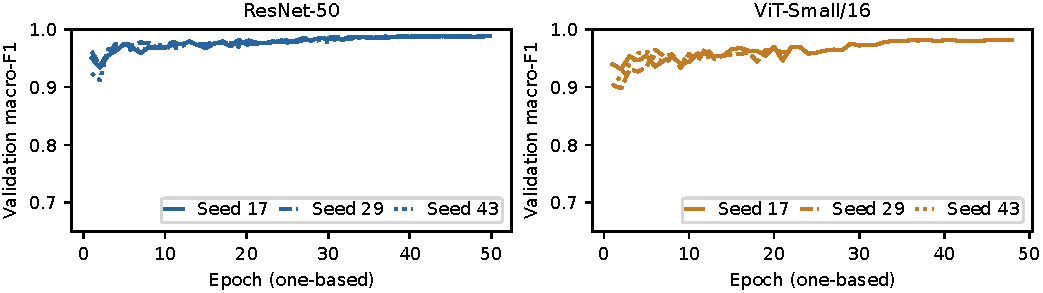
\includegraphics[width=\textwidth]{figures/learning_curves_compact.pdf}
\caption{Validation macro-F1 from the original training event logs. Line styles distinguish the three seeds within each model. Epochs are one-based, and the vertical scale spans 0.65--1.00. All points are validation measurements.}\label{fig:learning}
\end{figure}
\subsection{Optimization and recorded environments}
AdamW updates all trainable parameters with weight decay 0.05 and no label smoothing. A batch of 32 and two gradient-accumulation steps give an effective global batch of 64. Two warm-up epochs precede cosine decay, with a minimum learning-rate ratio of 0.01 and a maximum of 50 epochs. Early stopping uses validation macro-F1, patience ten, and minimum improvement 0.0001. Horizontal and vertical flips each have probability 0.5 and are deterministically keyed by source, epoch, and seed. Table~\ref{tab:models} gives the model-specific learning rates and representations.

The recorded ResNet environment uses Python 3.12.14, PyTorch 2.13.0, torchvision 0.28.0 and CUDA 13.0. The ViT environment uses Python 3.12.3, PyTorch 2.6.0+cu124, torchvision 0.21.0+cu124 and CUDA 12.4. Both record NumPy 1.26.4, SciPy 1.17.1, scikit-learn 1.9.0, Pillow 12.3.0, PyYAML 6.0.3 and Weights \& Biases 0.29.0. These versions describe the environments in the experiment artifacts; the manuscript-build runtime is documented separately. GPU precision resolved to bfloat16.

\section{Full Condition Summaries}
The following table reports mean $\pm$ sample SD across three training seeds. Each condition has 4,050 source images per seed. Raw cosine measures feature similarity within a model. ECDF instability places the corresponding dissimilarity in the validation different-class-control distribution. Bold marks the better model within each family-severity pair: higher accuracy, consistency, and raw cosine, or lower ECDF instability. Displayed ties are bold for both models. A value rounded to zero does not establish semantic invariance. The original condition and class CSVs in \path{supplementary/} retain full-precision per-seed values.
\begin{center}\resizebox{\textwidth}{!}{\input{tables/full_conditions.tex}}\end{center}
\subsection{Sham and control interpretation}
All three family shams have label consistency one in the stored summaries. Tiny representation differences from floating-point identity processing do not indicate an intervention effect. Different-class controls come from the source's evaluation partition and define the dissimilarity reference. Amplitude-mixing donors come from training and share the source's dataset label. Neither sham rows nor different-class controls enter the RQ3 positive class; shams are excluded from that task entirely.

The archived class-condition table retains the ten dataset classes, whose sample counts differ (Appendix~\ref{app:counts}). The separate macro-cluster confusion table groups classes for exploratory visualization. Those groups leave the training labels unchanged and have not been independently validated as a semantic taxonomy.

\subsection{Auxiliary artifacts and selection boundaries}
The archived cross-model CKA table uses one clean representation per source, paired by training-seed identifier. CKA compares sets of representations and does not establish semantic equivalence of individual image pairs. The supplementary directory retains the full original PNG and CSV collection. The following sections document gallery selection and attention rollout.

\section{High-Confidence Failures under Mild RGB Gains}\label{app:qualitative}
The gallery shows four correct-to-incorrect transitions under mild RGB gains. Each clean prediction agrees with the dataset label and has confidence at least 0.99. After transformation, the prediction switches between PermanentCrop and HerbaceousVegetation. Figures~\ref{fig:gallery1} and~\ref{fig:gallery2} retain the original sources and their recorded order.

Selection followed a deterministic rule. Eligible rows met the frozen condition policy, used mild RGB-gain or amplitude-mixing severity, had clean confidence at least 0.99, and exhibited a correct-to-incorrect transition. Rows were sorted by decreasing clean confidence, then by model, source and pair identifiers. The first four unique sources were retained. All four selected rows were RGB-gain failures. Replaying selection across all six runs reproduced the archived metadata. Since the examples were chosen for specific failure properties, they cannot estimate prevalence or represent every transformation family.

Original RGB files and transformed float32 caches were recovered from the migration backup. Their SHA-256 values match the dataset manifest and evaluation rows. The panels preserve the native 64-by-64 pixels. Confidence values are rounded to six decimal places; values close to one should not be read as certainty. The transformed images have not been independently re-annotated.
\begin{figure}[H]
\centering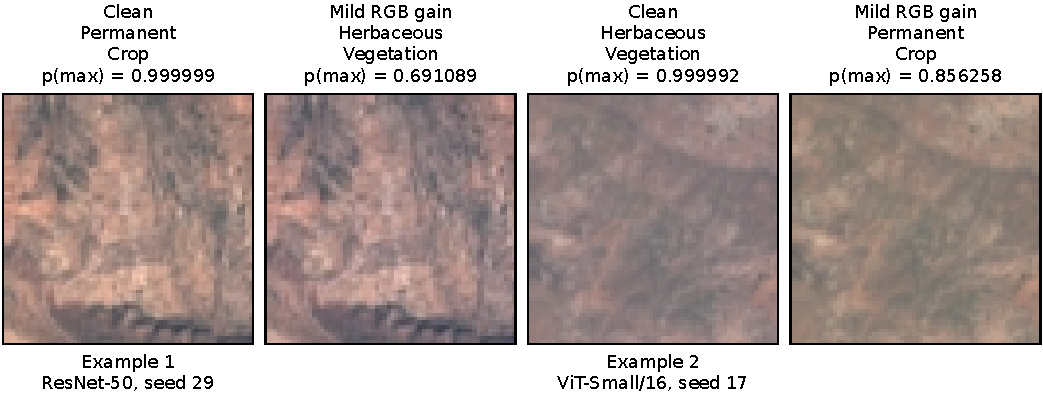
\includegraphics[width=\textwidth]{figures/qualitative_failure_gallery_1_compact.pdf}
\caption{Selected failures, examples 1 and 2, shown as two adjacent clean/transformed pairs. ResNet-50 seed29 changes from PermanentCrop to HerbaceousVegetation; ViT-Small/16 seed17 changes in the opposite direction. Each pair shows the clean input first and its recorded mild RGB-gain input second. Titles give predicted classes and maximum-softmax confidence. Clean predictions equal the dataset labels; run identifiers appear below the clean panels.}\label{fig:gallery1}
\end{figure}
Figure~\ref{fig:gallery2} continues the same deterministic selection with examples 3 and 4.
\begin{figure}[H]
\centering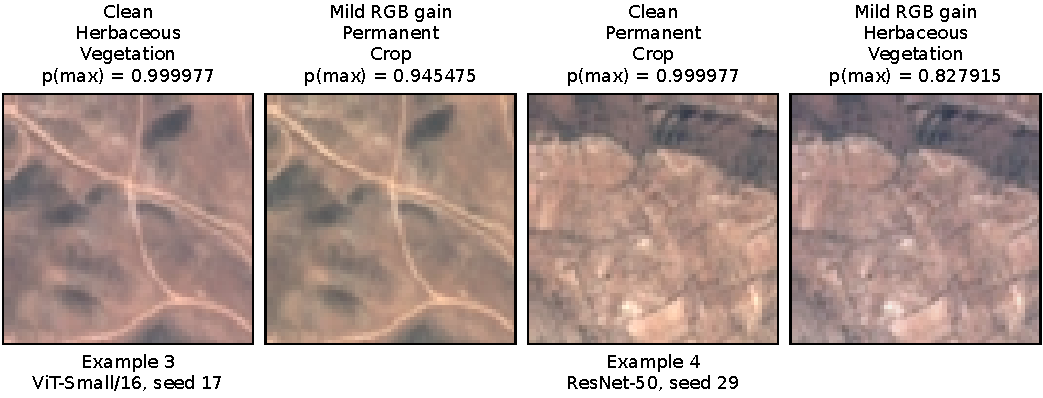
\includegraphics[width=\textwidth]{figures/qualitative_failure_gallery_2_compact.pdf}
\caption{Selected failures, examples 3 and 4, continuing the deterministic ordering in Figure~\ref{fig:gallery1} with two different sources. ViT-Small/16 seed17 predicts PermanentCrop for the transformed HerbaceousVegetation source; ResNet-50 seed29 predicts HerbaceousVegetation for the transformed PermanentCrop source. Correctness is measured against the original dataset labels.}\label{fig:gallery2}
\end{figure}
\FloatBarrier
\subsection{Interpreting the examples}
The selected pairs show class switches despite mild channel gains and high starting confidence. Their apparent visual similarity cannot establish that the original labels remain appropriate. They illustrate the benchmark's failure definition; the quantitative tables describe performance across the full evaluated populations. Example 2 is also the source selected by the archived ViT attention routine.
\section{Attention Rollout and Rendering Repair}\label{app:attention}
Attention rollout averages heads, adds identity connections, normalizes rows, and propagates attention through successive layers to approximate token information mixing~\cite{rollout}. The ViT-Small/16 seed17 example uses classification-token-to-patch rollout for gallery example 2. Each patch map is interpolated to 224-by-224 and min--max normalized separately. Rollout describes attention propagation without establishing causal pixel importance. Separate normalization also prevents interpreting color intensity as an absolute difference between clean and transformed attention.

The original plot overlays a 224-by-224 attention map on a 64-by-64 image without a shared extent. The coordinate mismatch compresses the image into one corner of the overlay. The supplementary materials preserve that PNG as a historical artifact; the figure below uses corrected coordinates.

The corrected rendering uses the same frozen ViT-Small/16 seed17 checkpoint and clean/transformed inputs. The local runtime uses \path{timm==1.0.29}, matching the recorded model-library version. One CPU forward call processed the two inputs. Both predicted classes match the archived pair, and the largest absolute difference in maximum confidence is 0.000153, below the predeclared 0.005 tolerance. The input and rollout layers share a 224-by-224 display extent. Figure~\ref{fig:attention} was visually checked at its original PNG resolution. No training, detector fitting or full-test inference was repeated.
\begin{figure}[H]
\centering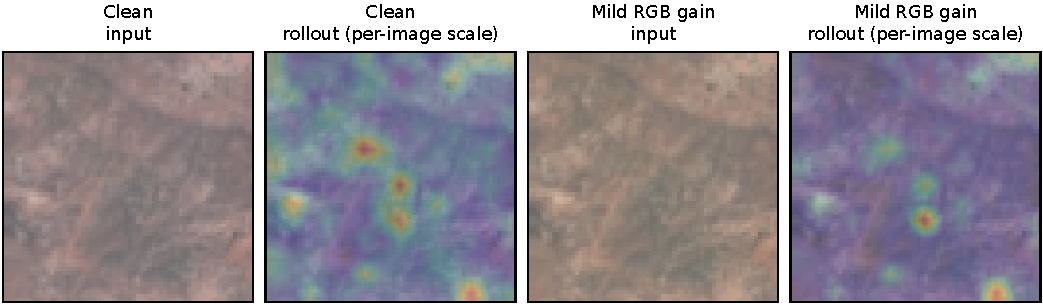
\includegraphics[width=\textwidth]{figures/attention_rollout_compact.pdf}
\caption{Corrected attention rollout for gallery example 2 using the frozen ViT-Small/16 seed17 checkpoint. The prediction changes from HerbaceousVegetation on the clean input to PermanentCrop under mild RGB gain. Panels show the clean input, clean rollout, transformed input, and transformed rollout in that order. The 64-by-64 inputs and overlays share the same coordinates. Each map is min--max normalized separately. Colors describe relative attention within each image and cannot establish an absolute change between images, causal pixel importance, or semantic label preservation.}\label{fig:attention}
\end{figure}
\section{Failure-Detector Populations and Paired Intervals}\label{app:detector}
Each eligible clean-correct source contributes nine non-sham pairs. The table below gives the resulting populations for every model and seed. Differences in failure prevalence affect the interpretation of AP even though each source receives the same nine conditions.
\begin{center}\input{tables/population.tex}\end{center}
The stored primary 95\% percentile intervals use 2,000 source-group bootstrap replicates. Both detector scores share every resampled row. The intervals are conditional on the trained checkpoint, fitted calibration detector, and fixed condition mixture, excluding uncertainty from detector refitting. They have not been adjusted for simultaneous coverage. Bold marks the largest gain for each metric within each model; interval bounds are not ranked.
\begin{center}\input{tables/delta_ci.tex}\end{center}
The gains compare the output-only baseline of transformed uncertainty and entropy with the same detector augmented by normalized representation instability. They apply to this feature comparison. Absolute per-seed scores and their uncertainty are available in \path{supplementary/detector_metrics.csv}; condition prevalence is in \path{supplementary/rq3_condition_prevalence.csv}. The primary tables report AP and AUROC separately and distinguish seed SD from the bootstrap intervals above.

\subsection{Exploratory analyses}
The archived exploratory table contains 36 defined tests across six model/seed runs, three families, and two configured metrics. Benjamini--Hochberg adjustment applies across that exploratory family, separately from the primary Holm procedure. The additional JS--ECDF Spearman correlations in \path{audit/relationships.json} were calculated after final evaluation from saved non-sham rows. Pooling severities within each run/family and repeating sources can induce association. The correlations are descriptive, without significance tests or causal interpretation.
\section{Provenance, Repairs, and Reproduction Boundaries}\label{app:provenance}
The following SHA-256 identifiers authenticate the recorded experiment. Labels and digests occupy separate lines for readability, and the machine-readable audit preserves the full strings. Repository availability and artifact authentication remain separate checks.
\begin{itemize}
\setlength{\itemsep}{1pt}
\item \textbf{Experiment protocol:}\\[-2pt] \path{cd20ca70be0619e87b2422fa99f7601c9b86578e06475f15a385903c9ed134a9}
\item \textbf{Base configuration:}\\[-2pt] \path{cc73206d4ff490bebaa9440af5689decd4a93d08038df486dadd8dfe0deb449c}
\item \textbf{Active campaign:}\\[-2pt] \path{d6dd3cabca656ef4414b165d82de1d9f45a228418a25e84e696eab9f248c7e8b}
\item \textbf{Dataset manifest:}\\[-2pt] \path{aa110365b4ad49a955680e1f8972eccd5a199946a3327f2e6a78cca0d78ced9a}
\item \textbf{Split:}\\[-2pt] \path{c678399552a928652dfa8d11aaa1288d1528fb272a0a888418e76223c29a9f0c}
\item \textbf{ResNet pretrained weights:}\\[-2pt] \path{5d061a3c593d795bfe682d9b152bafbcf550579873492def3515b46db1189888}
\item \textbf{ViT pretrained weights:}\\[-2pt] \path{c20a91d93f4757b0f581519f21ad91a875cf041764873a7a5bccc8e36f360dbf}
\end{itemize}
\subsection{Historical report-index defect}
The original \path{reporting.py} validates each representation file against its run's evaluation index. A later loop loads each run's metric and pair files but does not reassign the representation-path variable before writing the source list. Consequently, five historical entries contain the sixth run's representation digest; only the final entry is correct. The defect affects the source list. Each evaluation retains its own representation matrix, authenticated against its corresponding index.

The audit hashes each file at its explicit run path, checks evaluation and statistics digests, verifies NPZ pair ordering, and recomputes cosine and ECDF values in batches. Clean accuracy, macro-F1, condition means, failure counts, primary simple effect estimates, and AP/AUROC for all five detector scores are independently recomputed from saved outputs. Stored bootstrap intervals are authenticated against the primary statistics and their inspected implementation; a full independent rerun of the bootstrap replicates was not performed. Original files, including the incorrect historical report index, are preserved. Corrected per-run hashes are recorded in \path{audit/source_audit.json}.

The archived software-fix note documents an earlier vocabulary repair. The report validator's population wording changed from ``accepted'' to ``selected'', with the frozen protocol preserved. Python compilation passed after the repair, but pytest was unavailable on the remote runtime. The note therefore provides no evidence that the full software test suite passed there.

\subsection{Available reproduction paths}
Document reproduction needs this directory and a LaTeX engine with IEEEtran. Rebuilding assets requires the authenticated \path{all_artifacts/} tree and Python analysis packages; the qualitative panels also need the eight source/cache files recorded in the visual audit. Full experiment reproduction additionally requires the raw dataset, pretrained checkpoint binaries, resolved training configuration, software environment, pair-generation code, and appropriate compute. Regenerating transformation caches requires matching inputs and implementation. Availability and publication of these external training dependencies must be checked separately from document compilation.

Manuscript preparation did not create a Git tag, push to a remote, launch training, or repeat final-test inference. The project repository is cited in the abstract. The local baseline tag is \path{sac-campaign-v1-final}; the course's \path{v1.0-final} still needs owner confirmation. The team supplied author names, affiliation, and email addresses. All authors must approve the final submission. Administrative checks are recorded in \path{audit/qa_status.md} alongside the quantitative audit status.

\subsection{Visual revision provenance}
The scatter retains every non-sham pair, giving 109,350 observations in each model panel. The severe-condition heatmap preserves the three-seed mean of every original class/condition cell while revising grouping, labels, and color scale. Gallery selection and source/cache hashes were checked before the four original image pairs were rendered as two figures. Original report PNGs remain unchanged. Appendix~\ref{app:attention} documents the corrected attention figure and the limited replay used to create it. Figure sources, input hashes, runtime details, and logo trims are recorded in \path{audit/visual_revision.json} and \path{audit/attention_repair_status.json}.

\end{document}
